\documentclass[11.5pt]{sig-alternate} % sets document style to sig-alternate
% packages
% typesetting
%\usepackage{dirtytalk} % typset quotations easier (\say{stuff})
\usepackage{hanging} % hanging paragraphs
\usepackage[defaultlines=3,all]{nowidow} % avoid widows
\usepackage[pdfpagelabels=false]{hyperref} % produce hypertext links, includes backref and nameref
\usepackage{xurl} % defines url linebreaks, loads url package
\usepackage{microtype}
%\usepackage{textcomp}
%\newcommand{\texttildemid}{\raisebox{0.4ex}{\texttildelow}}
% layout
\usepackage{enumitem} % control layout of itemize, enumerate, description
\usepackage{fancyhdr} % control page headers and footers
\usepackage{float} % improved interface for floating objects
%\usepackage{multicol} % intermix single and multiple column pages
% language
\usepackage[utf8]{inputenc} % accept different input encodings
\usepackage[english]{babel} % multilanguage support
% misc
\usepackage{graphicx} % builds upon graphics package, \includegraphics
%\usepackage{lastpage} % reference number of pages
%\usepackage{comment} % exclude portions of text (?)
\usepackage{xcolor} % color extensions
\usepackage[backend=biber, style=apa]{biblatex} % sophisticated bibliographies % necessary for HTML to display author info and date on abstract page
\usepackage{csquotes} % advanced quotations, makes biblatex happy
\usepackage{authblk} % support for footnote style author/affiliation
% tables and figures
\usepackage{tabularray}
%\usepackage{array} % extend array and tabular environments
\usepackage{caption} % customize captions in figures and tables (rotating captions, sideways captions, etc)
%\usepackage{cuted} % allow mixing of \onecolumn and \twocolumn on same page
\usepackage{multirow} % create tabular cells spanning multiple rows
%\usepackage{subfigure} % deprecated, support for manipulation of small figures
%\usepackage{tabularx} % extension of tabular with column designator "x", creates paragraph-like column whose width automatically expands
%\usepackage{wrapfig} % allows figures or tables to have text wrapped around them
%\usepackage{booktabs} % better rules
% dummy text
%\usepackage{blindtext} % blind text dummy text
%\usepackage{kantlipsum} % Kant style dummy text
\usepackage{lipsum} %lorem ipsum dummy text
% other helpful packages may be booktabs, longtable, longtabu, microtype

\pagestyle{fancy} % sets pagestyle to fancy for fancy headers and footers

% header and footer
% modern way to set header image
\renewcommand{\headrulewidth}{0pt} % defines thickness of line under header
\renewcommand{\footrulewidth}{0pt} % defines thickness of line above header
\setlength\headheight{80.0pt} % sets height between top margin and header image, effectively moves page contents down
\addtolength{\textheight}{-80.0pt} % seems to affect the lower height. maybe only works properly if footer numbers enabled?
\fancyhf{}
\fancyhead[CE, CO]{
\includegraphics[width=\textwidth]{headerImage.png}}
% footer
%\fancyfoot[LE,LO]{Article Title Here \\ DOI: }% left footer article title and doi
%\fancyfoot[CE,CO]{{}} % center footer empty
%\fancyfoot[RE,RO]{\thepage} % right footer page numbers
%\pagenumbering{arabic} % arabic (1, 2, 3) numbering in footer

\hypersetup{colorlinks=true,urlcolor=blue} % sets link color to blue
\urlstyle{same} % sets url typeface to same as rest of text

% set caption and figure to italics, label bold, left align captions, does not transfer to HTML
\captionsetup{labelfont=bf, font={large, it}, justification=raggedright, singlelinecheck=false}
\renewcommand\theContinuedFloat{\alph{ContinuedFloat}}

%this next bit is confusing, but essentially changes the width of the abstract. Seems to have been copied from this https://tex.stackexchange.com/questions/151583/how-to-adjust-the-width-of-abstract
\let\oldabstract\abstract
\let\oldendabstract\endabstract
\makeatletter %changes @ catcode to enable modification (in parsep)
\renewenvironment{abstract} %alters the abstract environment
{\renewenvironment{quotation}%
               {\list{}{\addtolength{\leftmargin}{1em} % change this value to add or remove length to the the default ?
                        \listparindent 1.5em%
                        \itemindent    \listparindent%
                        \rightmargin   \leftmargin%
                        \parsep        \z@ \@plus\p@}%
                \item\relax}%
               {\endlist}%
\oldabstract}
{\oldendabstract}
\makeatother %changes @ catcode to disable modification

% checks
% italics -
% links - 
% dashes -
% tildes - 
\begin{document}

\title{Effects of Inquiry-Based Instruction on Science Achievement for Students with Disabilities:  An Analysis of the Literature}

\author[1]{\large \color{blue}Karen L. Rizzo}
\author[1]{\large \color{blue}Jonte C. Taylor}

\affil[1]{Pennsylvania State University}

\toappear{}
%% ABSTRACT
\maketitle
\begin{@twocolumnfalse} 
\begin{abstract}
\item 
\textit{In comparison to the past, more students with disabilities are being included in the general education classroom for science instruction. Though inquiry-based instruction has not shown to be an effective practice for students with disabilities, it is vastly becoming the dominant practice in science education. The purpose of this review is to examine the effects of inquiry-based instruction on science achievement for students with disabilities. The twelve studies, meeting selection criteria, report improvement in science achievement using inquiry practices. The participants and settings, variations of inquiry-based instruction, science achievement measures, and teacher training were addressed in this review. Two major contributions have resulted from analyzing the twelve studies. First, students with disabilities require supports to participate in an inquiry-based lesson and demonstrate progress on science achievement measures. Second, science achievement improves when components of explicit instruction are utilized in both the general and special education setting for students with disabilities.}
\\ \\
Keywords: inquiry-based instruction, science achievement, students with disabilities
\end{abstract}
\end{@twocolumnfalse}

%% AUTHOR INFORMATION

\textbf{*Corresponding Author,Karen L. Rizzo }\\
\href{mailto: kleerizzo@gmail.com }{(kleerizzo@gmail.com)} \\
\textit{Submitted  Jan 3 2016}\\
\textit{Accepted Mar 31 2016} \\
\textit{Published online May 18 2016} \\
\textit{DOI:10.14448/jsesd.09.0001} \\
\pagebreak
\clearpage
\begin{large}
\section*{INTRODUCTION}

Science content knowledge and skills play an important role in an individual’s ability to function independently and within society.  Science instruction can contribute to an individual’s ability to live independently or with reduced supports.  It also provides access to a wider range of opportunities to participate in society including access to competitive employment in science-related fields. STEM careers are predicted to expand by 17\% from 2008 to 2018 in comparison to non-STEM related careers, which are likely to increase by 9.8\% and require a minimum education level of a bachelor’s degree (Vilorio, 2014).   

\subsection*{Science Instruction for Students with Disabilities}
 
Science education has historically focused on students acquiring factual information presented from a textbook by the general education teacher (Anderson, 2002; Pine, Aschbacher, Roth, Jones, McPhee, Martin, \& Foley, 2006; Scruggs, Mastropieri, Bakken, \& Brigham, 1993; Scruggs \& Mastropieri, 2007).  Traditional text-book driven science instruction has not been the best means for students with disabilities to learn science content.  From a science education prospective, inquiry-based science instruction has emerged as the primary instructional method to be used in the general education setting (Maroney, Finson, Beaver, \& Jensen, 2003; Scruggs et al., 1993; Scruggs \& Mastropieri, 2007).   

Inquiry-based science became synonymous with terms such as discovery learning, hands-on learning, activity-based instruction, and project-based instruction.  However, a clear, standardized definition of inquiry-based instruction does not exist in the literature.  Inquiry should be considered a set of interrelated processes by which scientists and students pose questions about the natural world and investigate phenomena (National Resource Council [NRC], 2006).  Students acquire content knowledge and develop a rich understanding of relevant concepts, principles, models, and theories (Courtade, Browder, Spooner, \& DiBiase, 2010; NRC, 2006).  Components of inquiry-based instruction as outlined by the Next Generation Science Standards (NGSS) include an emphasis on data, requirement of evidence to claims, and/or opportunities for argumentation and analysis (NGSS Lead States, 2013).  Based on Scruggs and Mastropieri’s (2007) definition and the NGSS components, inquiry-based instruction can operationally be observed as student-conducted experiments with the use of an inquiry-based instructional framework.  This framework may take form as an approach to the scientific method, problem solving procedure, or by five phases that allow students to engage, explore, explain, apply, and evaluate for science understanding (Bybee, 1989).  While researchers have attempted to precisely conceptualize the differences between inquiry-based instruction and terminology used interchangeable for it, Martin-Hansen (2002) has provided a continuum within the practices of inquiry-based instruction (see Figure 1).
 
\begin{figure}[ht]
     \centering
     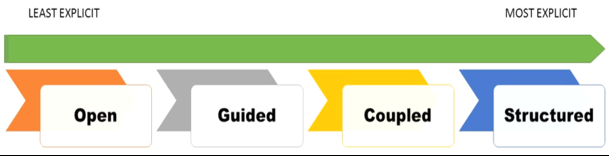
\includegraphics[width=1\linewidth]{fig1.png}
     \caption{ Inquiry-based instructional continuum arranged in usage from least to most explicit in instructional supports.  Adapted from “Defining inquiry: Exploring the many types of inquiry in the science classroom” by L. Martin-Hansen, 2002, Science Teacher, 69.  Copyright 2002 by The National Science Teachers Association. }
 \end{figure} 

Given the diverse needs of learners in the general education science classroom, the NRC (2006) revised its definition of inquiry-based instruction to include the minimal supports necessary to guide inquiry thus supporting the continuum of inquiry-based instruction.  Based on this information, the Martin-Hansen (2002) has outlined four distinct forms of inquiry-based instruction including: open inquiry, guided inquiry, coupled inquiry, and structured inquiry (Martin-Hansen, 2002).  Open inquiry is also referred to as full inquiry and most closely resembles actual scientific practice (Martin-Hansen, 2002).  It is as a student-centered approach where as the student directs the question, experiment, and communication of results.  Guided inquiry is more of a balanced approach of teacher and student direction through the investigative cycle with the teacher more directly addressing the development of inquiry skills.  Coupled inquiry is the combination of guided and open inquiry through the cycle of: inquiry, guided inquiry, open inquiry, resolution, and assessment (Martin-Hansen, 2002).  Lastly, structured inquiry is often referred to as directed inquiry and is often perceived as less engaging/student oriented and thus less effective (Martin-Hansen, 2002).  

Across the span of instructional practices of inquiry, there are distinct theoretical and practical application differences.  With the exception of structured inquiry, each of the other forms prioritize the conceptual change model of learning (Duit \& Treagust, 2003) in which guidance and support can be provided after the student has been given time to explore a new concept or skill.  The use of explicit instruction is not viewed as supporting true inquiry or cognitive engagement.  In contrast, structured inquiry provides supports, including components of explicit instruction, often from the start of instruction and faded overtime based on the ideas of behavioral momentum and practice of most-to-least prompting (Browder, Wood, Thompson, \& Ribuffo, 2014; Lee, Belfiore, Scheeler, Hua, \& Smith, 2004).  The concern for using structured inquiry seems to be centered around confusion over what constitutes active student engagement.  Regardless of theoretical discrepancies, it is important to reflect upon two key points found consistently within the literature base.  Previous research has suggested that inquiry-based instruction is mixed in its effectiveness.  Open inquiry based instruction is not recommended for students with disabilities (Samsonov, Pederson, \& Hill, 2006) however, dstructured inquiry has shown to be an effective teaching method for teaching science to students with learning disabilities (Therrien et al., 2011), emotional/behavioral disorders (Therrien et al., 2014) and students with autism and intellectual/developmental disabilities (Taylor et al., in preparation). 

\subsection*{Purpose of the Current Study}

Because inquiry-based instruction is becoming the dominant instructional approach to science instruction, it is logical to further investigate and determine how inquiry-based instruction impacts science achievement particularly for students with disabilities.

The purpose of this review is to evaluate the literature base on the use of inquiry-based science instruction for students identified as having a disability.  To that end, the researcher attempted to answer the following question and sub-questions:
\begin{enumerate}
    \item How effective is inquiry-based science instruction for students with disabilities?
\begin{enumerate} [label=(\alph*)]
    \item Who participated in each study and in what settings?
    \item How did the method inquiry-based instruction vary across each study?
    \item Did studies incorporate teacher training and professional development?  If so, did this contribute to the effect of inquiry-based instruction on science achievement?
\end{enumerate}
\end{enumerate}

\section*{METHODS}
\subsection*{Literature Search}

For this review, studies were located in a three-step process.  First, electronic databases were accessed through the Penn State University library system; the databases searched included: PsychINFO, Proquest, and Education Resources Information Center (ERIC).  The search was limited to peer-reviewed, scholarly journals with variations of the terms science, inquiry, and disability.  More specifically, the search included inquiry (OR inquiry-based OR inquiry-based instruction) AND (science OR science instruction OR science strategies OR science achievement) AND forms of the term disability.  The terms were narrowed to include: inquiry, “science achievement”, and disability for the purpose of locating studies specific to the main question of this review.  Next, an ancestral search was conducted based on the articles found across the three databases that met inclusionary criteria. The ancestral search reviewed both the articles which had cited the identified sources as well as the reference lists included by the identified sources for this review.  Third, a journal writer was contacted in order to locate unpublished studies, which led to a hand search on a special issue of Learning Disabilities Research \& Practice (2011).

\subsection*{Inclusion Criteria}

Included studies met four criteria.  First, participants in the study must include individuals diagnosed with a disability in accordance with IDEA, enrolled in a public, private, or other school setting (K-12).  Second, the articles had to be a peer-reviewed, empirical study using an experimental or quasi-experimental design.  Third, the article had to include a stated form of inquiry-based instruction as the independent measure.  Terms associated with inquiry were permitted including: inquiry-based, guided inquiry, supported inquiry, discovery, hands-on, project-based, and activity-based.  Fourth, the article had to measure science achievement as a dependent outcome. 

A total of 10 articles met the inclusionary criteria for this review following a search of the electronic databases.  An ancestral search of the references produced one additional study; an ancestral search showing where the original articles had been cited also provided one study for this review.  Information obtained via hand searches provided related information, but no articles from either resource was included here due to the specified criteria of this review.  Spanning across eight journals, twelve articles by different authors were identified as meeting the criteria for inclusion in this review of the literature.  

\subsection*{Analyses of Studies}

The researchers conducted a number of analyses during the review of the literature.  Descriptive analyses were conducted on the studies in the areas of participant and disability type, grade categories and settings, variations of inquiry-based instruction, achievement and assessment, and teacher training and professional development.  Component analyses were also conducted on components of inquiry-based instruction (Bybee, 1989; Magnusson \& Palincsar, 1995) and professional development standards (National Research Council [NRC], 1996).  Effect size was calculated for each study.

\subsection*{Effect Size Calculations}

Effect sizes for group design studies, was calculated using Hedges’s g.  Hedge’s g was used to account for the overestimation that occurs when calculating ES using studies with small sample sizes (Hedges, 1981).  As suggested by Cohen (1988), effect size interpretations should be large effects of .80 and above, medium effects at .50 to .80, and small effects at .50 and below.  For single case design studies, the percentage of non-overlapping data (PND) and Tau-U was calculated.  PND is calculated by determining the highest or lowest (depending on the intervention) data point in the baseline phase and how many points in the intervention phase exceed that point (Scruggs, Mastropieri, \& Casto, 1987).  Scruggs et al. (1987) suggest that PND should be considered most effective at 70\% or above, mildly effective between 50\% and 70\%, and no observable effect at 50\% or below. Tau-U was also calculated to show the percentage of non-overlap between phases controlling for positive baseline trend (Parker et al., 2011).  According to Parker and Vannest (2009), effect size interpretations should be large effects of .91-1.0, medium effects of .66-.92, and small effects of 0-.65.  

\section*{Results}

\subsection*{Effectiveness of Inquiry-based Instruction}

\subsubsection*{Descriptive statistics}
Across the twelve studies within this review, science achievement was measured using assessments created by experimenters, curriculum-based measures (CBMs), and one high stakes standardized assessment.  Additionally, one study piloted the Conservation of Matter Assessment (COMA), (Lynch et al., 2007).  Only Bay et al. (1992) used a performance-based assessment to measure generalization.  Eleven studies using guided or supported inquiry-based instruction were reviewed for how science achievement was measured.  Seven of these studies measured students’ content knowledge; five of these studies measured students’ application of concepts.  Furthermore, five studies focused specifically on vocabulary.  Of these eleven studies, five studies used experimenter developed assessments, three used CBMs, and one used a standardized assessment.  Overall, the studies report that students with disabilities made gains in the guided, or supported, inquiry-based conditions.

Overall, Bay et al. (1992) is the only study that examines the sole effects of inquiry-based instruction on science achievement for students with disabilities.  The results of Bay et al. (1992) do not reflect a higher gain in the discovery condition than the comparison condition using direct instruction on the post-test measure but does report a significant increase on generalization.  For these reasons, no studies within this review indicate that science achievement, for students with disabilities, improves using inquiry-based instruction.  Evidence from the remaining eleven studies analyzed in this review support the conclusion that components of explicit instruction support students with disabilities in an inquiry-based lesson.  In addition, components associated with explicit instruction supported an increase in science achievement specific to word identification and vocabulary acquisition for students with specific learning disabilities, autism spectrum disorder, intellectual disabilities, and multiple disabilities (Browder et al, 2012; Jimenez et al., 2012; Smith et al., 2013).

\subsubsection*{Effect size calculations}
Effect sizes were for all studies using PND and Tau-U for single case design studies and Hedge’s g for group design studies.  PND calculations for four single case design studies were conducted and yielded a range, that according to Scruggs et al. (1987), fall into the effective instruction range (70.19\% - 96.13\%) (See Table 4 for more detailed information).  TA-U calculations yielded a range, that according to Parker and Vannest (2009) and Rispoli et al. (2013), fall into both the medium-to-high effects of .66-.92 (Smith et al. 2013) and the large or strong effects range of .93-1.0 (Aydveniz et al., 2012; Courtade et al. 2010; Jimenez et al. 2013) (See Table 4 for more detailed information). Group design studies resulted in more variability regarding effectiveness.  Studies ranged in effect size from .44 to 2.992 (See Table 1).  Studies ranged from small effect to large effect (Cohen, 1988).

\subsection*{Participants, Disability Types, and Settings}

The researchers examined the participant information for each of the twelve studies included in this analysis.  Participant information consisted of the number of participants per study, the type of disabilities that participants had in each study, and the settings in which science instruction occurred.

\begin{table*}[htp]
\caption{Effect Sizes Per Study}
\begin{tabular}{lccc}
\hline
Study & & & Effect Sizes \\ \hline
& PND & Tau-U & Hedge’s g (95\% CI) \\ \hline
\textit{Single Case Studies} & & & \\ \hline
Aydveniz et al. (2012) & 86.75\% & 0.9985 & \\ \hline
Courtade et al. (2010) & 96.13\% & 0.9908 & \\ \hline
Jimenez et al. (2012) & 87.59\% & 0.931 & \\ \hline
Smith et al. (2013) & 70.19\% & 0.8693 & \\ \hline
\textit{Group Design Studies} & & & \\ \hline
Bay et al. (1992) & & & 2.992 (3.901, 2.082) \\ \hline
Browder et al. (2012) & & & 0.732 (6.410, -4.946) \\ \hline
Dalton et al. (1997) & & & 1.432 (3.906, 1.041) \\ \hline
Lynch et al. (2007) & & & 0.593 (4.056, -2.870) \\ \hline
Mastropieri et al. (2006) & & & ND\textsuperscript{a}\\ \hline
McCarthy (2005) & & & 2.471 (3.740, 1.202) \\ \hline
McCleery \& Tindal (1999) & & & 1.157 (1.0185, 1.295) \\ \hline
Scruggs et al. (1993) & & & 0.444 (-0.974, 1.861) \\ \hline
\end{tabular}
\textit{Note}.  PND = percent of non-overlapping data; CI = confidence interval; ND = not determined; \textsuperscript{a}Study did not provide enough information to determine effect size.
\end{table*}



\subsubsection*{Descriptive statistics}
Twelve studies, meeting inclusionary criteria, were included in this literature review with a total of 426 participants with disabilities. Studies were grouped by the following disability categories:  specific learning disabilities (Aydveniz Cihak, Graham, \& Retinger, 2012; Bay, Staver, Bryan, \& Hale, 1992; Dalton, Morocco, Tivnan, \& Mead, 1997; Mastropieri, Scruggs, Norland, Berkeley, McDuffie, Tornquist, \& Connors, 2006; McCarthy, 2005; McCleery \& Tindal, 1999; \& Scruggs et al., 1993);  intellectual disabilities (Browder, Trela, Courtade, Jimenez, Knight, \& Flowers, 2012; Courtade, Browder, Spooner, \& DiBiase, 2010; Jimenez, Browder, Spooner, \& DiBiase, 2012; McCarthy, 2005; \& Smith, Spooner, Jimenez, \& Browder, 2013);  emotional/behavioral disabilities (Bay et al., 1992; Mastropieri et al., 2006; \& McCarthy, 2005);  autism spectrum disorder (Aydveniz et al., 2012);  multiple disabilities (Smith et al., 2013); attention deficit hyperactivity disorder (McCarthy, 2005); and non-specified (Lynch, Taymans, Watson, Ochsendorf, Pyke, \& Szesze, 2007) (See Table 2 for more detailed information).  

\begin{table*}[htp]
\caption{Participant Details by Disability Type}
\begin{tabular}{lccc}
\hline
Disability Type & \# of Studies & \# of Participants & \% of Participants \\ \hline
Learning Disabilities & 7 & 130 & 30.6\% \\ \hline
Intellectual Disabilities & 5 & 40 & 9.4\% \\ \hline
Emotional/Behavioral Disabilities & 3 & 28 & 6.6\% \\ \hline
Autism Spectrum Disorders & 1 & 11 & 2.6\% \\ \hline
Multiple Disabilities & 1 & 2 & .47\% \\ \hline
Attention Deficit/Hyperactivity & 1 & 12 & 2.8\% \\ \hline
No Specified Disability & 1 & 202 & 47.5\% \\ \hline
\end{tabular}
\end{table*}

Although the majority of studies were conducted in the middle grades, 1st through 12th grades were represented with five studies implemented in elementary schools, seven studies implemented in middle schools, and one study implemented in a high school.  Three educational settings were represented in this review including general education classrooms, special education classrooms, and one hospital related setting (See Table 3).

\begin{table*}[h]
\caption{Grade Categories, Study Settings, and Inquiry Types}
\begin{tabular}{|l|c|c|c|}
\hline
Study & Grade Category & Study Setting & Inquiry Types \\ \hline
Aydveniz et al. (2012) & EL & SPLED & G \\ \hline
Bay et al. (1992) & MS \& HS & SPLED & O \\ \hline
Browder et al. (2012) & MS \& HS & SPLED & S \\ \hline
Courtade et al. (2010) & MS & SPLED & G \\ \hline
Dalton et al. (1997) & EL & GEN & G \\ \hline
Jimenez et al. (2012) & MS & GEN & S \\ \hline
Lynch et al. (2007) & MS & GEN & G \\ \hline
Mastropieri et al. (2006) & MS & GEN & G \\ \hline
McCarthy (2005) & MS & HOSP & G \\ \hline
McCleery \& Tindal (1999) & EL & GEN & S \\ \hline
Scruggs et al. (1993) & MS & GEN & G \\ \hline
Smith et al. (2013) & EL & SPLED & S \\ \hline
\end{tabular}
\textit{Notes}. EL= elementary; MS= middle school; HS= high school; GEN= general education; SPLED= special education; HOSP= partial hospitalization program; O= open inquiry; G= guided inquiry; C= coupled inquiry: S= structured inquiry.
\end{table*}

\subsection*{Variations of Inquiry-based Instruction}

Descriptive statistics and component analyses were conducted examining variations in inquiry-based instruction across studies.  Descriptive statistics provided results based on differences via type of inquiry.  Component analyses examined the implementation of inquiry-based instruction across studies based on the suggestions from Bybee et al. (1989) and Magnusson \& Palincsar, (1995).

\subsubsection*{Descriptive statistics}
Of the twelve studies, only Bay et al. (1992) used open inquiry-based instruction as an intervention aimed to promote science achievement for students with emotional/behavioral disorders or specific learning disabilities.  Students conducted experiments independent of teacher input.  The majority of the studies implemented a guided approach to inquiry-based instruction (Aydveniz et al., 2012; Courtade et al., 2010; Dalton et al., 1997; Lynch et al., 2007; Mastropieri et al., 2006; McCarthy, 2005; \& Scruggs et al., 1993). Aydveniz et al. (2012) and McCarthy (2005) each used components of explicit instruction to review vocabulary prior to the student-conducted experiments.  Priming techniques were also implemented (Aydveniz et al., 2012; Courtade et al., 2010; Dalton et al., 1997; Lynch et al., 2007; McCleery et al., 1999; and Scruggs et al., 1993) to enhance student recall of background information; these techniques included questioning related to background knowledge, student experiences, and key vocabulary.  Coaching, guided practice, shaping, and/or prompting techniques used in explicit instruction are present in the studies conducted by Courtade et al., (2010), McCarthy (2005), Dalton et al. (1997), and Lynch et al. (2007). 

None of the studies reviewed implemented a coupled approach to inquiry-based instruction.  The remaining four studies used a structured approach to inquiry-based instruction (Browder et al., 2012; Jimenez et al., 2012; McCleery \& Tindal, 1999; \& Smith et al., 2013).  Smith et al. (2013) and McCleery and Tindal (1999) each specify the application of explicit instruction as part of the independent variable.  Smith et al. (2013) used explicit instruction of concepts from the Early Science Curriculum; McCleery \& Tindal (1999) used explicit rule-based instruction for teaching the scientific method.  Like Aydveniz et al. (2012), McCarthy (2005) and Scruggs et al. (1993), Browder et al. (2012) also used components of explicit instruction to review vocabulary.  Priming techniques were used in ¾ structured inquiry studies similar to those implemented in studies using a guided approach.  Additionally, Scruggs et al. (1993) used the guided practice component of explicit instruction. 

\subsubsection*{Component Analyses}
Each study was evaluated based on the components of inquiry-based instruction implemented as suggested by previous researchers.  Two studies (Bay et al., 1992; Dalton et al., 1997) implemented components as suggested by Bybee et al. (1989).  Two studies (Browder et al., 2012; Courtade et al., 2010) implemented components as suggest by Magnusson \& Palincsar (1995).  All other studies did not specify the theoretical framework for inquiry-based instruction. In addition, studies were identified in terms of the type of inquiry-based instruction implemented according to the guidelines of open, guided, coupled, and structured (Martin-Hansen, 2002).  

\subsection*{Teacher Training/Professional Development}

\subsubsection*{Descriptive statistics}  
Of the twelve studies from this review, licensed practitioners with teaching experience ranging from 1.5 to 25 years carried out all interventions.  Dalton et al. (1997) and Lynch et al. (2007) had interventions carried out by general education teachers.  These teachers had no previous background knowledge or experience in special education.  Nine of the studies were carried out by special education teachers (Aydveniz et al., 2012; Browder et al., 2012; Courtade et al., 2010; Jimenez et al., 2012; Mastropieri et al., 2006; McCarthy, 2005; Scruggs et al., 1993; and Smith et al., 2013).  Of these only Aydveniz et al. (2012) and McCleery and Tindal (1999) were implemented by special education teachers with previous background knowledge on teaching science. Based on this information, special education teachers implemented the majority of studies with limited backgrounds in teaching science.

Component analysis of teacher training/profes\-sional development.  The NRC (1996) begins by describing six science-teaching standards. Each of the six science teaching standards described by the NRC (1996) is addressed in the studies examined by this review.  These standards are followed by standards for professional development in four main areas including: (a) science content knowledge, (b) pedagogy and science teaching, (c) life-long learning, and (d) coherent, integrated instruction with the standards.  Each study was evaluated on its use of the components for professional development and/or teacher training in science instruction (See Table 4).

\begin{table*}
\caption{Component Analysis of Professional Development by Study}
\begin{tabular}{|l|c|c|c|c|c|}
\hline
Study & \multicolumn{4}{|c|}{Professional Development Standards} & Notes \\ \hline
& a & b & c & d & \\ \hline
Aydveniz et al. (2012) & & & & & PD- Not provided \\ \hline
Bay et al. (1992) & & & & & PD- Not provided \\ \hline
Browder et al. (2012) & X & X & X & X & \\ \hline
Courtade et al. (2010) & X & X & X & X & \\ \hline
Dalton et al. (1997) & & & X & X & PD –Provided (NS) \\ \hline
Jimenez et al. (2012) & & & & & PD- Not provided \\ \hline
Lynch et al. (2007)& & X & X & & PD additional reform-based strategies \\ \hline
Mastropieri et al. (2006) & & & & & PD- Provided (NS) \\ \hline
McCarthy (2005) & & & & & PD- Not provided \\ \hline
McCleery \& Tindal (1999) & & & & & PD to teacher assistants for charting \\ \hline
Scruggs et al. (1993) & & & & & PD- Not provided \\ \hline
Smith et al. (2013) & & & & & PD- Not provided \\ \hline
\end{tabular}
\textit{Notes}. a = science content knowledge, b = pedagogy and science teaching, c = life-long learning, and d = coherent, integrated instruction with the standards, PD = professional development, PD NS = professional development mentioned but not specified.
\end{table*}

\section*{Discussion}

Science content knowledge and skills influence an individual’s quality of life and functioning within a society.  An individual’s health, safety, and independence can involve knowledge of science concepts (NSTA, 2004).  The skills acquired through science instruction include problem solving, critical thinking, and often collaboration.  Science instruction impacts fulfillment of high school graduation requirements and future employment opportunities.  Science instruction is critical to the development of a science literate society.  The importance of science for both individual and societal needs warrants examination of how science instruction is delivered particularly for individuals who require specialized instruction.

The purpose of this review was to examine the effects of inquiry-based instruction on science achievement for students with disabilities. Twelve articles implementing inquiry-based instruction were examined whose individual results stated support for inquiry-based instruction.  In order to examine the effect of inquiry-based instruction on science achievement for students with disabilities, studies were differentiated between those, which implemented open, guided, coupled, and structured inquiry-based instruction.  Next, science achievement measures were analyzed followed by an examination of teacher training and professional development on inquiry-based instruction.  The results of this review conclude that inquiry-based instruction, alone, was not supported by the literature as an effective approach to improve science achievement for students with disabilities.  The following section puts this information into context of the literature.  

\subsection*{Participants and Settings}

Based on the results of this review, inquiry-based instruction has been researched primarily with middle school students.  Of the total 427 participants across studies, nearly 75\% were identified as receiving special education services within the general education science classroom; It is worth noting that approximately half of the total participants from this review are from one particular study and the disability categories, of those participants, are non-specified (Lynch et al., 2007).  A majority of study participants with an identified disability category were found to have a learning disability and received inquiry-based instruction, equally, in the general and special education settings.  It can be concluded that inquiry-based instruction has been used in both the general and special education settings, grades 1-12, for students with a range of disabilities; however, it is important to note that the majority of these studies focused on supporting inquiry-based instruction.  These supports, whether guided or structured, were provided almost equally in both the general and special education setting.  It is also worth noting that the only study using open inquiry-based instruction for students with disabilities was conducted in the special education setting.

\subsection*{Variations of Inquiry-based Instruction}

Inquiry-based instruction was implemented independent of supports by Bay et al. (1992).  The remaining studies implemented inquiry-based instruction with supports.  Instead of providing supports in a reactive manner to student learning, Browder et al. (2012), Jimenez et al. (2012), McCleery and Tindall (1999), and Smith et al. (2013) provided components of explicit instruction proactively throughout the learning process.  In other words, the experimenters did not wait for students to construct their own meaning of the science concepts independently before providing supports.  If considering inquiry-based instruction as a continuum ranging from completely student-driven to completely teacher-driven instruction, there was one study that would be to the extreme of student-driven instruction (Bay et al., 1992) and only one study completely teacher-driven (McCleery \& Tindal, 1999); the remaining studies lie somewhere in between moving in one direction or another as support decreased or increased.  

\subsection*{Science Achievement}

Science achievement was primarily measured on the basis of experimenter-designed assessments; therefore, it is unclear on how these outcomes will transfer to a standardized, high-stakes measure.  Moreover, a significant amount of the testing was conducted outside the typical instructional environment therefore questions arise as to whether similar results would be obtained in the typical instructional/testing setting.  Additionally, only four of the studies measured maintenance and/or generalization.  The formats of the assessments were flexible offering a wide range of acceptable responses.  The types of questions required students to not only select responses but also often construct responses; these scores were obviously more qualitative and open to interpretation.  Multiple pre-test/post-test assessments were implemented across the twelve studies; concerns arise due to multiple exposures of the assessments.   In light of the variation of the testing instruments, assertions could not be made on any possible patterns, or discrepancies, that may be observed after multiple applications. 

Overall, science achievement seemed to improve when guided or structured inquiry was used based on the scope of this review.  Furthermore, results of the studies suggest that the greater the intensity of support, the more likely students with disabilities will yield gains in science achievement.  

\subsection*{Teacher Training/Professional Development}

Though the role of teacher training is significant to instructional practices, a relationship has not been established between teacher training and effects of inquiry-based instruction as evidenced by the majority of the studies in this review.  Only four of the studies describe, with detail, the professional development procedures needed for implementation (Browder et al., 2012; Courtade et al., 2010; Dalton et al., 1997; Lynch et al., 2007).  Surprisingly, of the nine studies implemented by special education teachers (individually or co-teaching) only three had either a background or professional development in the area of inquiry-based instruction (Aydveniz et al., 2012; Browder et al., 2012; \& Courtade et al., 2010).  Contrarily, of the five studies whose interventions were implemented by a general education teacher (individually or co-taught), none had any background or training in special education.  

\subsection*{Limitations of the Present Study}

There are also several limitations of this review.  First, the purpose of this review was to determine the effects of inquiry-based instruction on science achievement for students with disabilities. Only one study included in this review used inquiry-based instruction as an independent practice.  The packaging of inquiry-based instruction with other instructional practices makes it difficult to attribute any of the effects to one specific form of instruction to science achievement.  A second limitation is that no standard definition of inquiry-based instruction is present in the literature base; therefore, the definition of inquiry-based instruction that pertains to this review may or may not be generally agreed upon.  A third limitation of this review is the variance within the independent variables and a lack in standard application of inquiry-based instruction.  Finally, the use of PND as a measure of effect size for single case research has been criticized for exaggerating results (Banda \& Therrien, 2008).

\section*{CONCLUSION}

Inquiry-based instruction has been accepted as the primary approach for teaching science and the driving force in current science education reform initiatives; however, this review questions the research stating that it is an effective practice for students with disabilities due partially to the lack of consistency in how inquiry-based instruction has been defined, applied and interpreted and also to current trends in science achievement.  Current TIMSS and PISA results indicate that the United States falls 23rd in rank for science education programs and 29th in highest mean science scores across industrialized nations (Sedghi, Arnett, \& Chalabi, 2013).   Using the science achievement results from NAEP, there appears to have been a slight improvement in scores, for eighth grade students, from 2009 to 2011.  More specific to students with disabilities, the National Center of Educational Research (NCER, 2013) reports a significant achievement gap in science among students with disabilities and their typically achieving peers.

The National Science Foundation (NSF, 2003) states “students with disabilities are less likely than those without to graduate from high school, to enroll in college, and to graduate from college.”  The current state of science literacy and demands of the work force necessitate further research addressing science education for all students.

Eleven of the studies within this review examine how to support students with disabilities in an inquiry-based science classroom.  In doing so, the research fails to objectively seek out effective instructional practices.  Rather than asking how inquiry-based instruction effects science achievement for students with disabilities, the research reviewed has focused on how to support inquiry-based instruction.  When supports need to be added with the depth and degree found by the results of this review, it puts into question the effectiveness of inquiry-based instruction on science achievement for students with disabilities.  

It can be concluded from the studies represented in this review that supports for inquiry-based science instruction are necessary for students with disabilities to demonstrate progress on science achievement measures.  Students with a variety of disabilities, across 1st through 12th grades, were able to make higher gains on science achievement measures when components of explicit instruction were incorporated both in the general and special education setting.  These results clearly illustrate the importance of teachers’ knowledge of the learner when planning and implementing practices along the continuum of inquiry-based instruction.  The “one size fits all” approach to inquiry-based instruction fails to meet the needs of students with disabilities.  In order to effectively deliver instruction using the continuum of inquiry-based instruction, teacher training and professional development is critical to closing the achievement gap between students with and without disabilities.  It is exciting to see current STEM initiatives, seeking to improve science literacy in the U.S. and grow the future workforce, prioritizing the needs of all learners, specifically students with disabilities.  In the hope of contributing to the actualization of these goals, this review emphasizes the value of explicit instructional supports when teaching science to diverse learners using an inquiry-based framework.  

\end{large}
\clearpage
\section*{REFERENCES}\par 

\textit{References marked with an asterisk indicate studies included in the analysis.}

\leftskip 0.25in
\parindent -0.25in 

Anderson, R. D. (2002). Reforming science teaching: What research says about inquiry. \textit{Journal of science teacher education, 13}(1), 1-12.

*Aydeniz, M., Cihak, D. F., Graham, S. C., \& Retinger, L. (2012). Using inquiry-based instruction for teaching science to students with learning disabilities.  \textit{International Journal of Special Education, 27}(2), 189-206.

Banda, D. R., \& Therrien, W. J. (2008). A teacher's guide to meta-analysis. \textit{Teaching Exceptional Children, 41}(2), 66-71.

*Bay, M., Staver, J. R., Bryan, T., \& Hale, J. B. (1992). Science instruction for the mildly handicapped: Direct instruction versus discovery teaching. \textit{Journal of Research in Science Teaching, 29}(6), 555-570.

*Browder, D. M., Trela, K., Courtade, G. R., Jimenez, B. A., Knight, V., \& Flowers, C. (2012). Teaching mathematics and science standards to students with moderate and severe developmental disabilities.  \textit{Journal of Special Education, 46}(1), 26-35.

Bybee, R. W. (1989). Science and technology education for the elementary years: Frameworks for curriculum and instruction. \textit{The National Center for Improving Science Education}. Washington, D.C.: Office of Educational Research \& Improvement.

Cohen, J. (1988). Statistical power analysis for the behavioral sciences (2nd ed.).  Hillsdale, NJ: Lawrence Erlbaum.

*Courtade, G. R., Browder, D. M., Spooner, F., \& DiBiase, W. (2010). Training teachers to use an inquiry-based task analysis to teach science to students with moderate and severe disabilities. \textit{Education and Training in Autism and Developmental Disabilities, 45}(3), 378-399.

*Dalton, B., Morocco, C. C., Tivnan, T., \& Mead, P. L. R. (1997). Supported inquiry science teaching for conceptual change in urban and suburban science classrooms. \textit{Journal of learning disabilities, 30}(6), 670-684.

Hedges, L. V. (1981). Distribution theory for Glass's estimator of effect size and related estimators. \textit{Journal of Educational and Behavioral Statistics, 6}(2), 107-128.

*Jimenez, B. A., Browder, D. M., Spooner, F., \& Dibiase, W. (2012). Inclusive inquiry science using peer-mediated embedded instruction for students with moderate intellectual disability. \textit{Exceptional Children, 78}(3), 301-317. 

*Lynch, S., Taymans, J., Watson, W. A., Ochsendorf, R. J., Pyke, C., \& Szesze, M. J. (2007). Effectiveness of a highly rated science curriculum unit for students with disabilities in general education classrooms. \textit{Exceptional Children, 73}(2), 202-223.

Magnusson, S. J., \& Palincsar, A. S. (1995). The learning environment as a site of science education reform. \textit{Theory into Practice, 34}(1), 43-50.

Maroney, S. A., Finson, K. D., Beaver, J. B., \& Jensen, M. M. (2003). Preparing for Successful Inquiry in Inclusive Science Classrooms. \textit{Teaching Exceptional Children, 36}(1), 18-25.

Martin-Hansen, L. (2002).  Defining inquiry: Exploring the many types of inquiry in the science classroom.  \textit{The Science Teacher, 69}(2), 34-37.

*Mastropieri, M. A., Scruggs, T. E., Norland, J. J., Berkeley, S., McDuffie, K., Tornquist, E. H., \& Connors, N. (2006). Differentiated curriculum enhancement in inclusive middle school science effects on classroom and high-stakes tests.  \textit{The Journal of Special Education, 40}(3), 130-137.

*McCarthy, C. B. (2005). Effects of thematic‐based, hands‐on science teaching versus a textbook approach for students with disabilities. \textit{Journal of Research in Science Teaching, 42}(3), 245-263.

*McCleery, J. A., \& Tindal, G. A. (1999). Teaching the scientific method to at-risk students and students with learning disabilities through concept anchoring and explicit instruction. \textit{Remedial and Special Education, 20}(1), 7-18.

National Center for Education Statistics. (2013). Washington, DC: Institute of Education Sciences, U.S. Department of Education. Retrieved December 4, 2014, from \url{http://nces.ed.gov}

National Research Council. (1996). \textit{National science education standards}. Washington, DC: National Academy Press.

National Science Foundation, Division of Science Resources Statistics (2003). Women, minorities, and persons with disabilities in science and engineering.Arlington, VA (NSF 03-312).  Retrieved from \url{http://www.nsf.gov/statistics/nsf03312/c2/c2o.htm}

NGSS Lead States. (2013). Next Generation Science Standards: For States, By States.

Pine, J., Aschbacher, P., Roth, E., Jones, M., McPhee, C., Martin, C., \& Foley, B. (2006). Fifth graders' science inquiry abilities: A comparative study of students in hands‐on and textbook curricula. \textit{Journal of Research in Science Teaching, 43}(5), 467-484.

Samsonov, P., Pedersen, S., \& Hill, C. L. (2006). Using problem-based learning software with at-risk students: A case study. \textit{Computers in the Schools, 23}(1-2), 111-124.

Scruggs, T. E., \& Mastropieri, M. A. (2007). Science learning in special education: The case for constructed versus instructed learning. \textit{Exceptionality, 15}(2), 57-74.

*Scruggs, T. E., Mastropieri, M. A., Bakken, J. P., \& Brigham, F. J. (1993). Reading versus doing: The relative effects of textbook-based and inquiry-oriented approaches to science learning in special education classrooms. \textit{The Journal of Special Education, 27}(1), 1-15.

Scruggs, T. E., Mastropieri, M. A., \& Casto, G. (1987).  The quantitative synthesis of single-subject research methodology and validation. \textit{Remedial and special Education, 8}(2), 24-33.

Sedghi, A., Arnett, G., \& Chalabi, M. (2013). Pisa 2012 results: which country does best at reading, math and science. \textit{The Guardian. Retrieved October, 21}, 2015.

*Smith, B. R., Spooner, F., Jimenez, B. A., \& Browder, D. (2013). Using an early science curriculum to teach science vocabulary and concepts to students with severe developmental disabilities. \textit{Education and Treatment of Children, 36}(1), 1-31.

Therrien, W. J., Taylor, J. C., Hosp, J. L., Kaldenberg, E. R., \& Gorsh, J. (2011). Science Instruction for Students with Learning Disabilities: A Meta‐Analysis. \textit{Learning Disabilities Research \& Practice, 26}(4), 188-203.

Therrien, W. J., Taylor, J. C., Watt, S., \& Kaldenberg, E. R. (2014). Science instruction for students with emotional and behavioral disorders. \textit{Remedial and Special Education, 35}(1), 15-27.

Vilorio, D. (2014). STEM 101: Intro to tomorrow’s jobs. \textit{Occupational Outlook Quarterly, 58}(1), 2-12.

\end{document}
